\documentclass[12pt,fleqn]{article}
\usepackage{a4}
\usepackage{graphicx}
\usepackage{psfrag}
\usepackage{amsmath}                     % \boldsymbol{#1}
\usepackage{amssymb}

%\usepackage{hangcaption}
%\usepackage{Styles/pstricks}
%\usepackage{Styles/pst-node}
\usepackage{Styles/fancyheadings}
\usepackage{tocloft}
\usepackage[euler]{textgreek}
\usepackage{booktabs}
\usepackage{mhchem}
\usepackage{siunitx}
\usepackage{bm}
\usepackage{tabularx,ragged2e,rotating}
\newcolumntype{C}{>{\hspace{0pt}%
    \Centering\arraybackslash}X}
\usepackage[skip=0.333\baselineskip]{caption}
\usepackage{longtable}
\usepackage{pdflscape}
%\usepackage{mathtools}
%\usepackage{unicode-math}
%\setmathfont{XITS Math}
%\newcommand*{\matr}[1]{\mathbfit{#1}}
%\newcommand*{\tran}{^\mkern-1.5mu\mathsf{T}}}
%\newcommand*{\conj}[1]{\overline{#1}}
%\newcommand*{\hermconj}{^{mathsf{H}}}
\usepackage{MnSymbol}
\usepackage{pdfpages}
%\usepackage{breqn}
\usepackage{float}
\usepackage{nccmath}
%\usepackage{chngcntr}
%-----Tex width---------------------------------
\textwidth 16cm

%\counterwithout{figure}{chapter}

%-----Line spacing-------------------------------
\renewcommand{\baselinestretch}{1.5}     % 1,1-zeilig

%---------Add dots in TOC-----------------------
\renewcommand{\cftsecleader}{\cftdotfill{\cftdotsep}}

%------Paragraph indention-------------------------------
\setlength{\parskip}{1.5ex plus0.5ex minus0.5ex}

%-----Prevent indent----------------------
\setlength{\parindent}{0em}

%-----Richtiger Abstand fur Einheiten-------------
\def\Unit{\hspace{0.25em}}

%-----Definition of the header--------------------
\pagestyle{fancyplain}
\renewcommand{\sectionmark}[1]{\markboth{Chapter~\thesection.~#1}{#1}}
\renewcommand{\subsectionmark}[1]{\markright{\thesubsection\ #1}}
\rhead[\fancyplain{}{\leftmark}]%
{\fancyplain{\thepage}{\thepage}} \cfoot{} \plainheadrulewidth
0.4pt
%% Otherwise: Overfull \vbox-Warning against fancyheadings-pacakage
%%  idea of: nic@minster.york.ac.uk (Nick Cropper)
\makeatletter
\ifcase \@ptsize \relax % 10pt
  \addtolength{\headheight}{1\p@}
\or % 11pt
  \addtolength{\headheight}{2\p@}
\or % 12pt
  \addtolength{\headheight}{3\p@}
\fi \makeatother

%-----Equations / Figures / Tables numbering according to \ sections
\makeatletter
\renewcommand\theequation{\arabic{section}.\arabic{equation}}
\renewcommand\thefigure{\arabic{section}.\arabic{figure}}
\renewcommand\thetable{\arabic{section}.\arabic{table}}
\@addtoreset{equation}{section} \@addtoreset{figure}{section}
\@addtoreset{table}{section} \makeatother

%-----Useful abbreviations----------------------
\newcommand{\mr}{\mathrm}
%%\newcommand{\bs}[1]{\mbox{$\boldsymbol{#1}$}}
\newcommand{\degree}[1]{\mbox{$#1^\circ$}}

%\renewcommand{\figurename}{Bild}

%------Bibliography style-----------------------
\bibliographystyle{IEEEtran}

%-----Aufzaehlunstiefe im Literaturverzeichnis---------------
\setcounter{tocdepth}{3}

\begin{document}
\pagenumbering{Roman}
\begin{titlepage}
  \begin{center}
      \vspace*{-4.0cm}
    \begin{figure}[!h]
\centering
\includegraphics[width=0.3\linewidth]{Figures/JKUAT_logo}
%\caption{}
\label{fig:jomologo}
\end{figure}
   \large{Jomo Kenyatta University of Agriculture and Technology}\\
    \large{College of Engineering and Technology}\\
    \large{School of Mechanical, Materials, and Manufacturing Engineering}\\
   \large{Department of Mechatronic Engineering}\\

    ------------------------------------------------------------------------------------------------\\[0.1cm]
      \vspace{0.1cm}
        \LARGE{\textbf{Development of a 6 DOF Stewart platform
            Force Balance for a Low Speed Wind Tunnel}}\\
        \vspace{0.2cm}
        \LARGE{\large\textbf{FYP 18-9
                }}\\
        {\large\textbf{FINAL PROJECT REPORT
                    }}\\[0.1cm]
        %\large{by}\\[0.6cm
    
        \vspace{0.1cm}
        \large{\textbf{Sammy Kerata Oina (ENM221-0089/2017)
                }}\\
         \large{\textbf{Earl Spencer Mogire~(ENM221-0074/2017)
                }}\\[0.3cm]
        \large{\textbf{Supervisors}}\\
        \large{Dr. Anthony K. Muchiri
                    }\\
        \large{Ms. Maurine N. Andanje
                        }\\
        \large{\textbf{Technologist}}\\
                \large{Mr. J Mbugua
                            }\\
         %Submitted in partial fulfillment of the requirements for the degree of Bachelor of Science in Mechatronic Engineering in Jomo Kenyatta University of Agriculture and Technology, 2022.
    %     \large{\textbf{Supervisors}}\\
    %    \large{Dr.-Ing.~Jackson G. Njiri}\\
    %    \large{Prof. George N. Nyakoe}\\
    %    \large{\ldots}    \\[0.2cm]\vfill
        \large{\small{\today}}\\
        \small{Submitted in partial fulfillment of the requirements for the degree of Bachelor of Science in Mechatronic Engineering in Jomo Kenyatta University of Agriculture and Technology, 2022.}
    ------------------------------------------------------------------------------------------------\\[1.5cm]
  \end{center}
\end{titlepage}
%
%\pagenumbering{gobble}% Remove page numbers (and reset to 1)

\addcontentsline{toc}{section}{Declaration}
\section*{Declaration}

We hereby declare that the work contained in this report is original; researched and documented by the undersigned students. It has not been used or presented elsewhere in any form for award of any academic qualification or otherwise. Any material obtained from other parties have been duly acknowledged. We have ensured that no violation of copyright or intellectual property rights have been committed.
\begin{enumerate}
	\item Sammy Kerata Oina\vspace*{.2cm}\\
	Signature\ldots\ldots\ldots\ldots\ldots\ldots\ldots\ldots\ldots\ldots Date\ldots\ldots\ldots\ldots\ldots\ldots\ldots\ldots\ldots\ldots
	\item Earl Spencer Mogire\vspace*{.2cm}\\
	Signature\ldots\ldots\ldots\ldots\ldots\ldots\ldots\ldots\ldots\ldots Date\ldots\ldots\ldots\ldots\ldots\ldots\ldots\ldots\ldots\ldots
\end{enumerate}

\vspace*{.5cm}
Approved by supervisors:
\begin{enumerate}
	\item Dr. Anthony K. Muchiri \vspace*{.2cm}\\
	Signature\ldots\ldots\ldots\ldots\ldots\ldots\ldots\ldots\ldots\ldots Date\ldots\ldots\ldots\ldots\ldots\ldots\ldots\ldots\ldots\ldots
	%\item Prof. George N. Nyakoe\vspace*{.2cm}\\
	%Signature\ldots\ldots\ldots\ldots\ldots\ldots\ldots\ldots\ldots\ldots Date\ldots\ldots\ldots\ldots\ldots\ldots\ldots\ldots\ldots\ldots
	\item Ms. Maurine Andanje\vspace*{.2cm}\\
	Signature\ldots\ldots\ldots\ldots\ldots\ldots\ldots\ldots\ldots\ldots Date\ldots\ldots\ldots\ldots\ldots\ldots\ldots\ldots\ldots\ldots
\end{enumerate}



\clearpage
\addcontentsline{toc}{section}{Abstract}

\section*{Abstract}
\label{sec:Abstract}
Obtaining and simulating the aerodynamic performance of items in a wind tunnel is a
significant and important part of development of vehicles, aircraft and other machines
that require aerodynamic performance evaluation. Due to the complex maneuvers
that may require simulation, there is a need for dynamic positioning of the model of the object in the wind tunnel. As a result, the proposal for a Stewart platform to
replicate complex maneuvers during wind tunnel tests as well as to position the model to
obtain the required data.

This project will look into the modeling, simulation and development of a Stewart
platform based force balance for a small low speed wind tunnel. The project will utilize
MatLab/ Simulink for modeling and simulation as well as Autodesk inventor for the mechanical
design. A robust control system will also be developed for the Stewart platform.
Finally the project will be developed and tested in a wind tunnel to evaluate the performance
of the platform. The force balance and platform should be able position the test
item and measure forces as well as calculate the aerodynamic coefficients using a bespoke computer program.





\clearpage
\addcontentsline{toc}{section}{Table of Contents}
\tableofcontents
\clearpage
\addcontentsline{toc}{section}{List of Figures}
{
%
\let\oldnumberline\numberline%
\renewcommand{\numberline}{\figurename~\oldnumberline}%
\listoffigures
\clearpage
\addcontentsline{toc}{section}{List of Tables}
\renewcommand{\numberline}{\tablename~\oldnumberline}%
\listoftables 
\newpage
\clearpage
%\addcontentsline{toc}{section}{List of Abbreviations}
\paragraph{Nomenclature}
\begin{itemize}
    \item A - Cross-section area
    \item a - Diameter of moving
    \item b - Diameter of base
    \item B - coordinate system defined at centre of base plate
    \item COG - Center of Gravity
    \item d - length of rod
    \item DAQ/DAQA - Data Acquisition System
    \item DOF - Degrees of Freedom
    \item E - Young's Modulus
    \item EASA - East Africa School of Aviation
    \item ELB - Engineering Laboratory Building
    \item F - Axial Force
    \item FEA - Finite Element Analysis
    \item G - Modulus of rigidity
    \item $H$ - transformation matrix which related measured forces and applied forces
    \item h - height between base plate and moving platform
    \item HMI - Human Machine Interface
    \item I2C - Inter-Integrated Circuit
    \item J - Jacobian Matrix
    \item JKUAT - Jomo Kenyatta University of Agriculture and Technology
    \item NASA - National Space Agency
    \item RS - Recommended Standard
    \item SCL - Serial Clock
    \item SDA - Serial Data
    \item SPI - Serial Peripheral Interface
    \item TTL - Transistor-Transistor Logic
    \item UDP - User Datagram Protocol
\end{itemize}
\pagebreak
%\paragraph{List of Symbols
%\begin{itemize}
%\item $\vec{b}_i$ - position of ith connection point at base with respect to B
%\item $\vec{F}_e$ - external force applied to platform
%\item $f_i$ - force exerted on ith leg due $F_e, M_e$
%\item $F$ - vector of leg forces
%\item $\hat{I}_i$ - Unit vector along the ith leg
%\item $\vec{M}_e$ - external moment applied to platform
%\item $\hat{{S_{i}}}$ - unit vector of the Plucker coordinates
%\item $\alpha$ - Angle of attack
%\item $\beta$ - Side slip angle
%\item $|J|$ - determinant of Jacobian matrix
%\item $|J|_{m}$ - determinant of Jacobian matrix of optimal Stewart PLatform configuration
%\item $\lambda$ - Quaity index
%\end{itemize}}
\clearpage
\newpage
%\addcontentsline{toc}{section}{List of Symbols}
\section*{List of Symbols}
    $B_{k}$ - leg attachment on base\\
    $H_{k}$ - Servo horn anchor\\
    $\vec{b}_i$ - position of ith connection point at base with respect to B\\
    $\vec{F}_e$ - external force applied to platform\\
    $f_i$ - force exerted on ith leg due $F_e, M_e$\\
    $F$ - vector of leg forces\\
    $\hat{I}_i$ - Unit vector along the ith leg\\
    $\vec{M}_e$ - external moment applied to platform\\
    $\hat{{S_{i}}}$ - unit vector of the Plucker coordinates\\
    $\alpha$ - Angle of attack\\
    $\alpha_{k}$ - Servo angle\\
    $\beta$ - Side slip angle\\
    $\beta_{k}$ - servo rotation angle form plan view\\
    $\epsilon$ - Strain\\
    $|h|$ - distance between original base anchor and platform anchor\\
    $|J|$ - determinant of Jacobian matrix\\
    $|J|_{m}$ - determinant of Jacobian matrix of optimal Stewart Platform configuration\\
    $\lambda$ - Quality index\\
    $l_{k}$ - leg length\\
    $P_{k}$ - leg attachment on platform\\
    $^{p}R_{b}$ - Rotation of the platform\\
    $R_{y}$ - rotation about y-axis\\
    $R_{z}$ - rotation about z-axis\\
    $\sigma$ - Stress\\
    $^{p}T_{b}$ - translation from the base origin to the platform origin\\
    $t_{x}$ -  translation in the x direction\\
    $t_{y}$ -  translation in the y direction\\
    $t_{z} $ -  translations in the z direction\\
\pagebreak
\clearpage
\newpage

\newpage
\pagenumbering{arabic}
  \section{Introduction}
\label{sec:introduction}
\subsection{Background}
\paragraph{}Research on Fuel cells started in 1801 when British Chemist Humphry Davy was setting up experiments to assist him in separating several materials using voltaic piles. The experiments set the background for the development of fuel cells which Christian Friedrich Schönbein worked on in 1838. Sir William Grove was the first scientist to prove that reaction between hydrogen and oxygen produced electricity in 1939. He carried out experiments on water electrolysers and fuel cells using his background on electrolysis to come up with a reverse process to generate electricity. He succeeded in building a device that combined water and hydrogen to generate electricity. The new device was originally called a gas battery, but later was renamed the fuel cell.
\paragraph{}The first operational fuel cell was developed by Charles Langer and Ludwig Mond. The duo developed a functional fuel cell, obtaining fuel capacity of 0.73V at 20A/m2. Francis Bacon advanced the Mond and Langer fuel cell in 1958, which was later used in the Apollo mission in 1969. Since then, the space agencies have been using fuel cells to power the space crafts and provide water for the astronauts.
\begin{figure}
\includegraphics{Figures/Figure3}
\caption{Fuel Cell Structure
\cite{pukrushpan_modeling_2003}}
\end{figure}

\paragraph{}With the current global challenge in the energy sector, there is an increasing need for power generation with minimal pollution and environmental degradation. As a way of mitigating environmental pollution and providing energy shortage routes, Fuel Cell technologies have been considered as elements of alternative energy systems. These technologies capitalize on high efficiencies (between 50–65 percent, Supramaniam, et al., 1999 \cite{ashby_fuel_nodate}) and low emissions.
\paragraph{}Fuel cells are increasingly becoming a promising alternative to internal combustion engines (ICEs) and thus are considered for transportation (automotive, marine and aerospace) applications. They are also being considered for distributed power generation for residential homes and industries. Another promising use of FC stacks is for electricity storage in conjunction with electrolyzers and hydrogen accumulators.\cite{stefanopoulou_mechatronics_nodate}
\paragraph{}Power generation from Fuel Cells (FC) necessitates the integration of chemical, fluid,
mechanical, thermal, electrical, and electronic subsystems. This integration presents many
challenges and opportunities in the mechatronics engineering field. A fuel cell system is made up of a water and heat management system, an air system, a humidifier system and a hydrogen in-out let system. For optimum operation of the Fuel cell, some factors must be controlled - these are: the hydrogen flow, air supply, water cooling temperature, membrane temperature and humidity. Control strategies are therefore imminent so that the FC operates within some established limits such as electric power, pressure of the fuel gas and amount of air for the anode chemical reaction.
\paragraph{}There are several types of fuel cells, each using a different chemistry. The common types of fuel cells are:
\begin{itemize}
\item Polymer electrolyte fuel cells
\item Direct methanol fuel cells
\item Alkaline fuel cells
\item Phosphoric acid fuel cells
\item Solid oxide fuel cells
\item Reversible fuel cells
\item Molten carbonate fuel cells
\end{itemize}
\paragraph{}Polymer electrolyte fuel cells and alkaline fuel cells were the commonly used fuel cells for space missions. Development of fuel cells for commercial activities started in 2007, with an interest to develop fuel cells for automobile applications. The Polymer Electrolyte membrane (PEM) fuel cell is commonly used to power vehicles. Currently, the Polymer Electrolyte Membrane (PEM) Fuel Cells (also known as Proton Exchange Membrane Fuel Cells) are considered by many to be in a relatively more developed stage for ground vehicle applications. PEM Fuel Cells have high power density, solid electrolyte, long cell and stack life, as well as low corrosion. They have greater efficiency when compared to heat engines and their use in modular electricity generation and propulsion of electric vehicles is promising \cite{holze_supramanian_2007}. This proposal will focus on the design and development of a control system for a Proton Exchange Membrane Fuel Cell (PEMFC).

\subsection{Basic Operation Principle of a Hydrogen  Fuel Cell}
\begin{figure}[!h]
\includegraphics{Figures/Figure1}
\caption{Fuel cell types and their respective operating temperatures
\cite{stefanopoulou_mechatronics_nodate}}
\end{figure}
\begin{figure}[!h]
\includegraphics{Figures/Figure2}
\caption{Fuel Cell Reactions
\cite{pukrushpan_modeling_2003}}
\end{figure}
\paragraph{}Fuel cells convert chemical energy sources directly to electricity. A fuel cell consists of an electrolyte sandwiched between two electrodes. The electrolyte has a special property which allows protons to pass through while blocking electrons. Hydrogen gas passes over one electrode, i.e. an anode, and with the help of a catalyst, separates into electrons and hydrogen protons.
\begin{equation}
$$2H_{2}\rightarrow 4H^{+} + 4e^{-}$$
\end{equation}
\paragraph{}The protons flow to the other cathode through the electrolyte while the electrons flow through an external circuit, thus creating electricity. The hydrogen protons and electrons combine with oxygen flow through the cathode, and produce water.
\begin{equation}
$$O_{2}+ 4H_{2} + 4e^{-} \rightarrow 2H_{2}O $$
\end{equation}
\paragraph{}The overall reaction of the fuel cell is given by:
\begin{equation}
$$2H_{2}+ O_{2} \rightarrow 2H_{2}O $$
\end{equation}

\subsection{Problem statement}
\paragraph{}As a measure to curb pollution due to the industrialization and transportation sectors, world governments are turning to alternative sources of energy. These alternative sources of energy should drastically reduce the pollution rates by cutting down emissions. Fuel cell technology is one such example of alternative sources of energy. A fuel cell uses the chemical energy of hydrogen or other fuels to cleanly and efficiently produce electricity. Moreover, fuel cells can operate at higher efficiencies than combustion engines and can convert the chemical energy in the fuel directly to electrical energy with efficiencies capable of exceeding 60\%. Fuel cells have lower or zero emissions compared to combustion engines.
\paragraph{}The various departments of energy, however,  have to work closely with national laboratories, universities, and industry partners to overcome critical technical barriers to fuel cell development. These barriers are cost, performance, and durability which are still key challenges in the fuel cell industry. 
\paragraph{}This design proposal seeks to provide a solution to improving the fuel cell’s performance by improving the robustness and efficiency of the Fuel Cell stack system for real world conditions through precise control of reactant flow and pressure, stack temperature, and membrane humidity\cite{stefanopoulou_mechatronics_nodate}.
\subsection{Objectives}
\subsubsection{Main Objectives}
\begin{enumerate}
\item To develop a Hydrogen Fuel cell control system.
\end{enumerate}
\subsubsection{Specific Objectives}
\begin{enumerate}
\item To design and additively manufacture a PEMFC prototype which can be adapted for domestic use and scaled for industrial applications.
\item To design and fabricate supporting control electronics for the Hydrogen Fuel Cell.
\item To achieve precise control of reactant flow and pressure, stack temperature, and membrane humidity.
\item To simulate and test alternative control strategies for the Hydrogen fuel cell. 
\end{enumerate}
\subsection{Justification of the study}
\paragraph{}Additive manufacturing offers the ability to produce intricate products and parts with lower development costs, shorter lead times, less energy consumed during manufacturing as well as less material waste. This method can be used to manufacture delicate components such as the bipolar plates with elimination of the risks involved such as breakage of brittle graphene material during production.     
\paragraph{}Precise control of reactant flow and pressure, stack temperature, and membrane humidity will increase the fuel cell’s robustness as well as efficiency \cite{stefanopoulou_mechatronics_nodate}\cite{gonzatti_proposal_2017}\cite{thanapalan_model_nodate}.
\paragraph{}The goal of this research is to develop physic-based dynamic models of fuel cell systems and fuel processor systems and then apply multivariable control techniques to study their behavior. The analysis will give insight into the control design limitations and provide guidelines for the necessary controller structure and system re-design.
  \clearpage
  \section{Literature Review}
\subsection{Force Balances}
\paragraph{}For wind tunnel applications, the wind axes is used as the reference frame. Where, X axis points to the accelerated air; Z axis points downward and; Y axis points to the right in the direction of the wind. In the reference frame above, lift is in the negative z-direction, drag in the negative x-direction and, side force in the negative y-direction.
\paragraph{}Moment components on the x,y,z axes are rolling moment, pitching moment and yawing moment respectively. A three-component force balance can be considered to measure the lift, drag and pitch (angle of attack).
\paragraph{}Force balances can be external or internal. In external force balances the test section lies outside of the wind tunnel test section, whereas in internal force balances the balance is inside the model itself connecting the model to the support structure.
\paragraph{}Several different types of external force balances are available for wind tunnel use
\cite{morris_force_2010}:
\begin{enumerate}
\item Wire
\item Platform
\item Yoke
\item Pyramidal
\end{enumerate}
\begin{center}
	\begin{figure}[!h]
	\centering
	\includegraphics{Figures/Fig6}
	\caption{Typical configurations for external force balances}
	\end{figure}
\end{center}
\paragraph{}In the wire balance, the model under testing is suspended by wires each connected to an extensometer (a sensor that produces an electrical output when submitted to a load and deforms). The shortcoming of the wire balance is the large tare drag caused by the wires which is difficult to quantify. They are also not robust nor versatile enough compared with the other alternatives. 
\paragraph{}The platform balance is relatively easy to construct, assemble and instrument. However, for this balance, forces and torques are coupled and the balance resolving center does not coincide with the center of the tunnel. 
\paragraph{}In the yoke balance configuration, forces and torques are coupled and the balance resolving center coincides with the center of the tunnel. This configuration, however, presents some structural deflections due to the large span of the measuring and support arms.
\paragraph{}The pyramidal balance configuration is a further improvement of the yoke balance in order to overcome the shortcomings of the other balances. It is capable of measuring six components of forces and
torques separately and without coupling,provided that the balance is well assembled and calibrated.

\paragraph{}The different kinds of internal balances can be made based on:
\begin{enumerate}
\item The type of transducer i.e. strain gauge or piezoelectric balance.
\item Shape i.e. box balance and sting balance
\end{enumerate} 
\begin{center}
	\begin{figure}[!h]
	\centering
	\includegraphics{Figures/Fig7}
	\caption{Typical configurations for internal force balances. \textit{Left to right:} Box balance and sting balance.}
	\end{figure}
\end{center}
\paragraph{}The box balance presents a cubic shape and can either be made of a solid piece of material or from assembled parts. In this configuation, the loads are transferred from the top to the bottom. The sting balance presents a cylindrical shape and the loads are transferred from one end to the other in the longitudinal direction. It can be used to measure forces or torques.
\paragraph{}The advantage of internal force balances is that they minimize the interference caused by the supporting bars in the flow.
\subsection{Sensors}
\subsubsection{Load Sensors}
\paragraph{}Several methods can be used to measure forces and torques in a force balance. These methods can be generally grouped into two:
\begin{enumerate}
\item Hydraulic measuring techniques.
\item Electric measurement techniques.
\end{enumerate}
\paragraph{}Electric measurement techniques are preferred for Force balance applications. One such electric measurement device is the strain gauge. A strain gauge is an electromechanical device whose electrical resistance changes linearly with the strain in the component.
\paragraph{}Metal foil strain gauges are widely used. This type of strain gauge provide more precise strain values than wire strain gauges. However, since the relative changes on electric resistance of the strain gauge are so small, it is necessary to develop an effective method to measure them because each strain gauge would require extremely accurate signal measurements. The solution is to have a set of strain gauges coupled in order to minimize the required accuracy, forming a force transducer i.e. the \textit{Wheatstone bridge}.
	\begin{figure}[!h]
	\includegraphics{Figures/Fig9}
	\caption{Wheatstone Bridge Circuit}
	\end{figure}
\paragraph{}Load cells can also be used to measure the drag and lift forces.
\subsubsection{Altitude Sensor}
\paragraph{}It is important to define the desired aerodynamic angles and to guarantee that they are measured accurately in relation to the air stream. One such angle is the angle of attack (\textalpha) shown in Figure 2.4. For this reason, specific devices that provide the attitude measurement should be implemented in order to improve the precision of the results.
\paragraph{}Angle of attack (\textalpha)- angle measured between the longitudinal axis of the model and the direction of the flow on a vertical (Figure 2.4)
\begin{center}
	\begin{figure}[!h]
	\centering
	\includegraphics{Figures/Fig10}
	\caption{Angle of attack (\textalpha)}
	\end{figure}
\end{center}
  \clearpage
    \section{Methodology}
\subsection{Force Sensor}
\paragraph{}The force sensor module will be used to measure the force and moments from the aerodynamic loads applied on model being tested in the wind tunnel. The forces to be measured are the drag, lift and thrust as well as associated moments. For this subsystem two possible conceptual designs are to be considered:
\begin{itemize}
\item External force sensor
\item Stewart Platform as a force sensor
\end{itemize}
\subsubsection{External Force Sensor}
\paragraph{}In this case it would require at least 3 orthgonally positioned load cells measuring each force component. Each load cell would be mechanically linked to the model such that forces experienced on each axis are measured by each load cell. 
\begin{center}
	\begin{figure}[!h]
		\centering
		\includegraphics{Figures/modBal}
		\caption{Diagram of a force balance \cite{post_force_2010}}
	\end{figure}
\end{center}
\paragraph{} This configuration is however bulky by requiring an additional external system for force measurements in addition to the stewart platform for positioning the model. This is however complemented by the simplicity in calibration of the load cells and does not require a complex force transformation matrix and other issues with force amplification created by the use of an integrated system.
\subsubsection{Stewart Platform as a force sensor}
\paragraph{} In this configuration the stewart platform legs are used as force sensors by attaching strain gauges in the legs of platform. Similar work has been done by \cite{ferreira2015design} without the use of actuators as is proposed in this project. Using the stewart platform as a force sensor requires the actuators to be locked with zero degrees of freedom.
\paragraph{} Four strain gauges are required for each leg for a full wheatstone bridge configuration. 
\begin{center}
	\begin{figure}[!h]
		\centering
		\includegraphics{Figures/loadConf}
		\caption{Strain Gauge Configuration \cite{noauthor_measuring_nodate}}
	\end{figure}
\end{center}
\paragraph{}In this case as shown in the figure the load cells are able to measure the axial strain on each leg. R1 and R3 are active strain gauges measuring the compressive Poisson effect (–νe). R2 and R4 are active strain gages measuring the tensile strain (+e). The output generated from the wheatstone bridge is then amplified and read to determine the strain on each leg.
\paragraph{Force transformation matrix}
In such a case the forces experienced at the top of the platform are distributed between the 6 legs and as result, a force transformation matrix is required to resolve the forces apllied on each axis as measured by each load cell on each leg. 
\paragraph{} If the platform is acted upon by an external wrench {$\vec{F}_e, \vec{M}_e$}, for static equilibrium of the body, the external wrench is statically balanced by the six leg forces of the stewart platform. Representing the unit vector $\hat{I}_i$ along the i-th leg with respect to B, the leg force is given  by $\hat{I}_if_i$. Considering the force equilibrium of the platform along  three mutually perpendicular directions in B(XYZ), the following force equations can be obtained:
\paragraph{}$(F_e)_x = f_1I_{1x} + f_2I_{2x} + f_3I_{3x} + f_4I_{4x} + f_5I_{5x} + f_6I_{6x}$
\paragraph{}$(F_e)_y = f_1I_{1y} + f_2I_{2y} + f_3I_{3y} + f_4I_{4y} + f_5I_{5y} + f_6I_{6y}$
\paragraph{}$(F_e)_z = f_1I_{1z} + f_2I_{2z} + f_3I_{3z} + f_4I_{4z} + f_5I_{5z} + f_6I_{6z}$
\paragraph{} where $(F_e)_x$, $(F_e)_y$ and $(F_e)_z$ are the external forces on the platform along three mutually perpendicular directions x, y and z of the frame B, respectively.
\paragraph{} The moment due to the forces $\hat{I}_if_i$ about the origin of B is $(\vec{b}_i x \hat{I}_i)f_i$. Considering the moment equilibrium about x, y and z axes of B, the following moment equations can be obtained:
\paragraph{}$(M_e)_x = f_1(\vec{b}_1 x \hat{I}_1)_x + f_2(\vec{b}_2 x \hat{I}_2)_x + f_3(\vec{b}_3 x \hat{I}_3)_x + f_4(\vec{b}_4 x \hat{I}_4)_x + f_5(\vec{b}_5 x \hat{I}_5)_x + f_6(\vec{b}_6 x \hat{I}_6)_x$
\paragraph{}$(M_e)_y = f_1(\vec{b}_1 x \hat{I}_1)_y + f_2(\vec{b}_2 x \hat{I}_2)_y + f_3(\vec{b}_3 x \hat{I}_3)_y + f_4(\vec{b}_4 x \hat{I}_4)_y + f_5(\vec{b}_5 x \hat{I}_5)_y + f_6(\vec{b}_6 x \hat{I}_6)_y$
\paragraph{}$(M_e)_z = f_1(\vec{b}_1 x \hat{I}_1)_z + f_2(\vec{b}_2 x \hat{I}_2)_z + f_3(\vec{b}_3 x \hat{I}_3)_z + f_4(\vec{b}_4 x \hat{I}_4)_z + f_5(\vec{b}_5 x \hat{I}_5)_z + f_6(\vec{b}_6 x \hat{I}_6)_z$
where $(M_e)_x$, $(M_e)_y$ and $(M_e)_z$ are the external moments on the platform  about the three coordinate axes of B. Combining the equations the relationship between the external wrench and the forces experienced by the legs can be expressed as follows:
$$
\begin{Bmatrix}
\vec{F}_e \\
\vec{M}_e \\
\end{Bmatrix} = [H]\{F\}
$$
  \clearpage
    \section{Expected Outcomes}
\begin{enumerate}
\item A fuctional stewart platform with six degrees of freedom postioning of a model within a wind tunnel.
\item A functional force sensor for measuring the aerodynamic load applied on a model and calculate aerodynamic coefficients from the meaurements taken.
\item An improved velocity measurement system for the wind tunnel using pitot tubes.
\item A human Machine Interface with access to control  of the stewaart platform electronics and data aquisition from sensors.
\end{enumerate}
\newpage
\subsection{Proposed Budget}
\begin{center}
\begin{table}[!h]
\centering
\caption{Proposed budget}
\paragraph{ }
\includegraphics{Figures/budget}
\end{table}
\end{center}
\subsection{Work Plan}
\begin{center}
\begin{table}[!h]
\centering
\caption{Workplan table}
\paragraph{ }
\includegraphics[width=0.95\linewidth]{Figures/workplan}
\end{table}
\end{center}

  \clearpage
    \chapter{Conclusion}
\begin{enumerate}
\item A six-DOF Stewart platform has been designed. This platform can achieve 3 linear and 3 angular movements. It has a high quality index i.e. 0.86 and is therefore mechanically feasible.
\item From Finite Element Analysis, the six legs of the Stewart platform experience significant strains which can be used to obtain force measurements during model testings in Wind Tunnel experiments.
\end{enumerate}



%  \clearpage
 %\input{Files/Summary}
  \clearpage
%----  Bibliography  ----------------------------------------
\markright{References}                               % Erzeugt Kopfzeile
\addcontentsline{toc}{section}{References}            % Literaturverzeichnis ins Inhaltsverzeichnis
%\bibliographystyle{Bib/IEEEtran}
\bibliography{Bib/References}                         % BIBTeX
\nocite{Lun01} 

                                     % Falls etwas in die Literaturliste soll, was nicht Referenziert wird
\newpage
\clearpage
\appendix
%\addcontentsline{toc}{section}{Appendices}
\section{Appendices}
\pagenumbering{roman}
\subsection{Stewart Platform and Wind Tunnel Configurations}
\includepdf[pages=-]{Wind Tunnel Assembly + Stewart}
\includepdf[pages=-]{Assemby 3 2}
\clearpage
\subsection{Budget and TimePlan}
\subsubsection{Provisional Budget}
\begin{center}
	\begin{table}[H]
		\centering
		\caption{Proposed budget}
		\paragraph{ }
		\includegraphics{Figures/budget}
	\end{table}
\end{center}
\subsubsection{Work Plan}
\begin{center}
	\begin{table}[H]
		\centering
		\caption[Time plan]{Time plan for first and second semester}
		\paragraph{ }
		\includegraphics[width=0.95\linewidth]{Figures/workplan}
	\end{table}
\end{center}
\clearpage
\subsection{Production Plan}
\includepdf[pages=-]{Production plan}

\clearpage

\subsection{Force transformation matrix}
In such a case the forces experienced at the top of the platform are distributed between the 6 legs and as result, a force transformation matrix is required to resolve the forces applied on each axis as measured by each load cell on each leg.

If the platform is acted upon by an external wrench {$\vec{F}_e, \vec{M}_e$}, for static equilibrium of the body, the external wrench is statically balanced by the six leg forces of the Stewart platform. Representing the unit vector $\hat{I}_i$ along the i-th leg with respect to B, the leg force is given  by $\hat{I}_if_i$. Considering the force equilibrium of the platform along  three mutually perpendicular directions in B(XYZ), the following force equations can be obtained as in \cite{dwarakanath_design_2001}:

\begin{ceqn}
	\begin{align}
		(F_e)_x = f_1I_{1x} + f_2I_{2x} + f_3I_{3x} + f_4I_{4x} + f_5I_{5x} + f_6I_{6x}
	\end{align}
\end{ceqn}
\begin{ceqn}
	\begin{align}
		(F_e)_y = f_1I_{1y} + f_2I_{2y} + f_3I_{3y} + f_4I_{4y} + f_5I_{5y} + f_6I_{6y}
	\end{align}
\end{ceqn}
\begin{ceqn}
	\begin{align}
		(F_e)_z = f_1I_{1z} + f_2I_{2z} + f_3I_{3z} + f_4I_{4z} + f_5I_{5z} + f_6I_{6z}
	\end{align}
\end{ceqn}
where $(F_e)_x$, $(F_e)_y$ and $(F_e)_z$ are the external forces on the platform along three mutually perpendicular directions x, y and z of the frame B, respectively.

The moment due to the forces $\hat{I}_if_i$ about the origin of B is $(\vec{b}_i x \hat{I}_i)f_i$. Considering the moment equilibrium about x, y and z axes of B, the following moment equations can be obtained as in \cite{dwarakanath_design_2001}:

\begin{ceqn}
	\begin{align}
		(M_e)_x = f_1(\vec{b}_1 x \hat{I}_1)_x + f_2(\vec{b}_2 x \hat{I}_2)_x + f_3(\vec{b}_3 x \hat{I}_3)_x + f_4(\vec{b}_4 x \hat{I}_4)_x + f_5(\vec{b}_5 x \hat{I}_5)_x + f_6(\vec{b}_6 x \hat{I}_6)_x
	\end{align}
\end{ceqn}
\begin{ceqn}
	\begin{align}
		(M_e)_y = f_1(\vec{b}_1 x \hat{I}_1)_y + f_2(\vec{b}_2 x \hat{I}_2)_y + f_3(\vec{b}_3 x \hat{I}_3)_y + f_4(\vec{b}_4 x \hat{I}_4)_y + f_5(\vec{b}_5 x \hat{I}_5)_y + f_6(\vec{b}_6 x \hat{I}_6)_y
	\end{align}
\end{ceqn}
\begin{ceqn}
	\begin{align}
		(M_e)_z = f_1(\vec{b}_1 x \hat{I}_1)_z + f_2(\vec{b}_2 x \hat{I}_2)_z + f_3(\vec{b}_3 x \hat{I}_3)_z + f_4(\vec{b}_4 x \hat{I}_4)_z + f_5(\vec{b}_5 x \hat{I}_5)_z + f_6(\vec{b}_6 x \hat{I}_6)_z
	\end{align}
\end{ceqn}

where $(M_e)_x$, $(M_e)_y$ and $(M_e)_z$ are the external moments on the platform  about the three coordinate axes of B. Combining the equations the relationship between the external wrench and the forces experienced by the legs can be expressed as follows:
\begin{ceqn}
	\begin{align}
		\begin{Bmatrix}
			\vec{F}_e \\
			\vec{M}_e \\
		\end{Bmatrix} = [H]\{F\}
	\end{align}
\end{ceqn}
\clearpage
\subsection{Code}
The complete firmware and HMI programs can be found in this repository,

https://github.com/SammyOina/stewart-platform.
\clearpage

\subsection{PCB schematics}
\subsubsection{schematics}
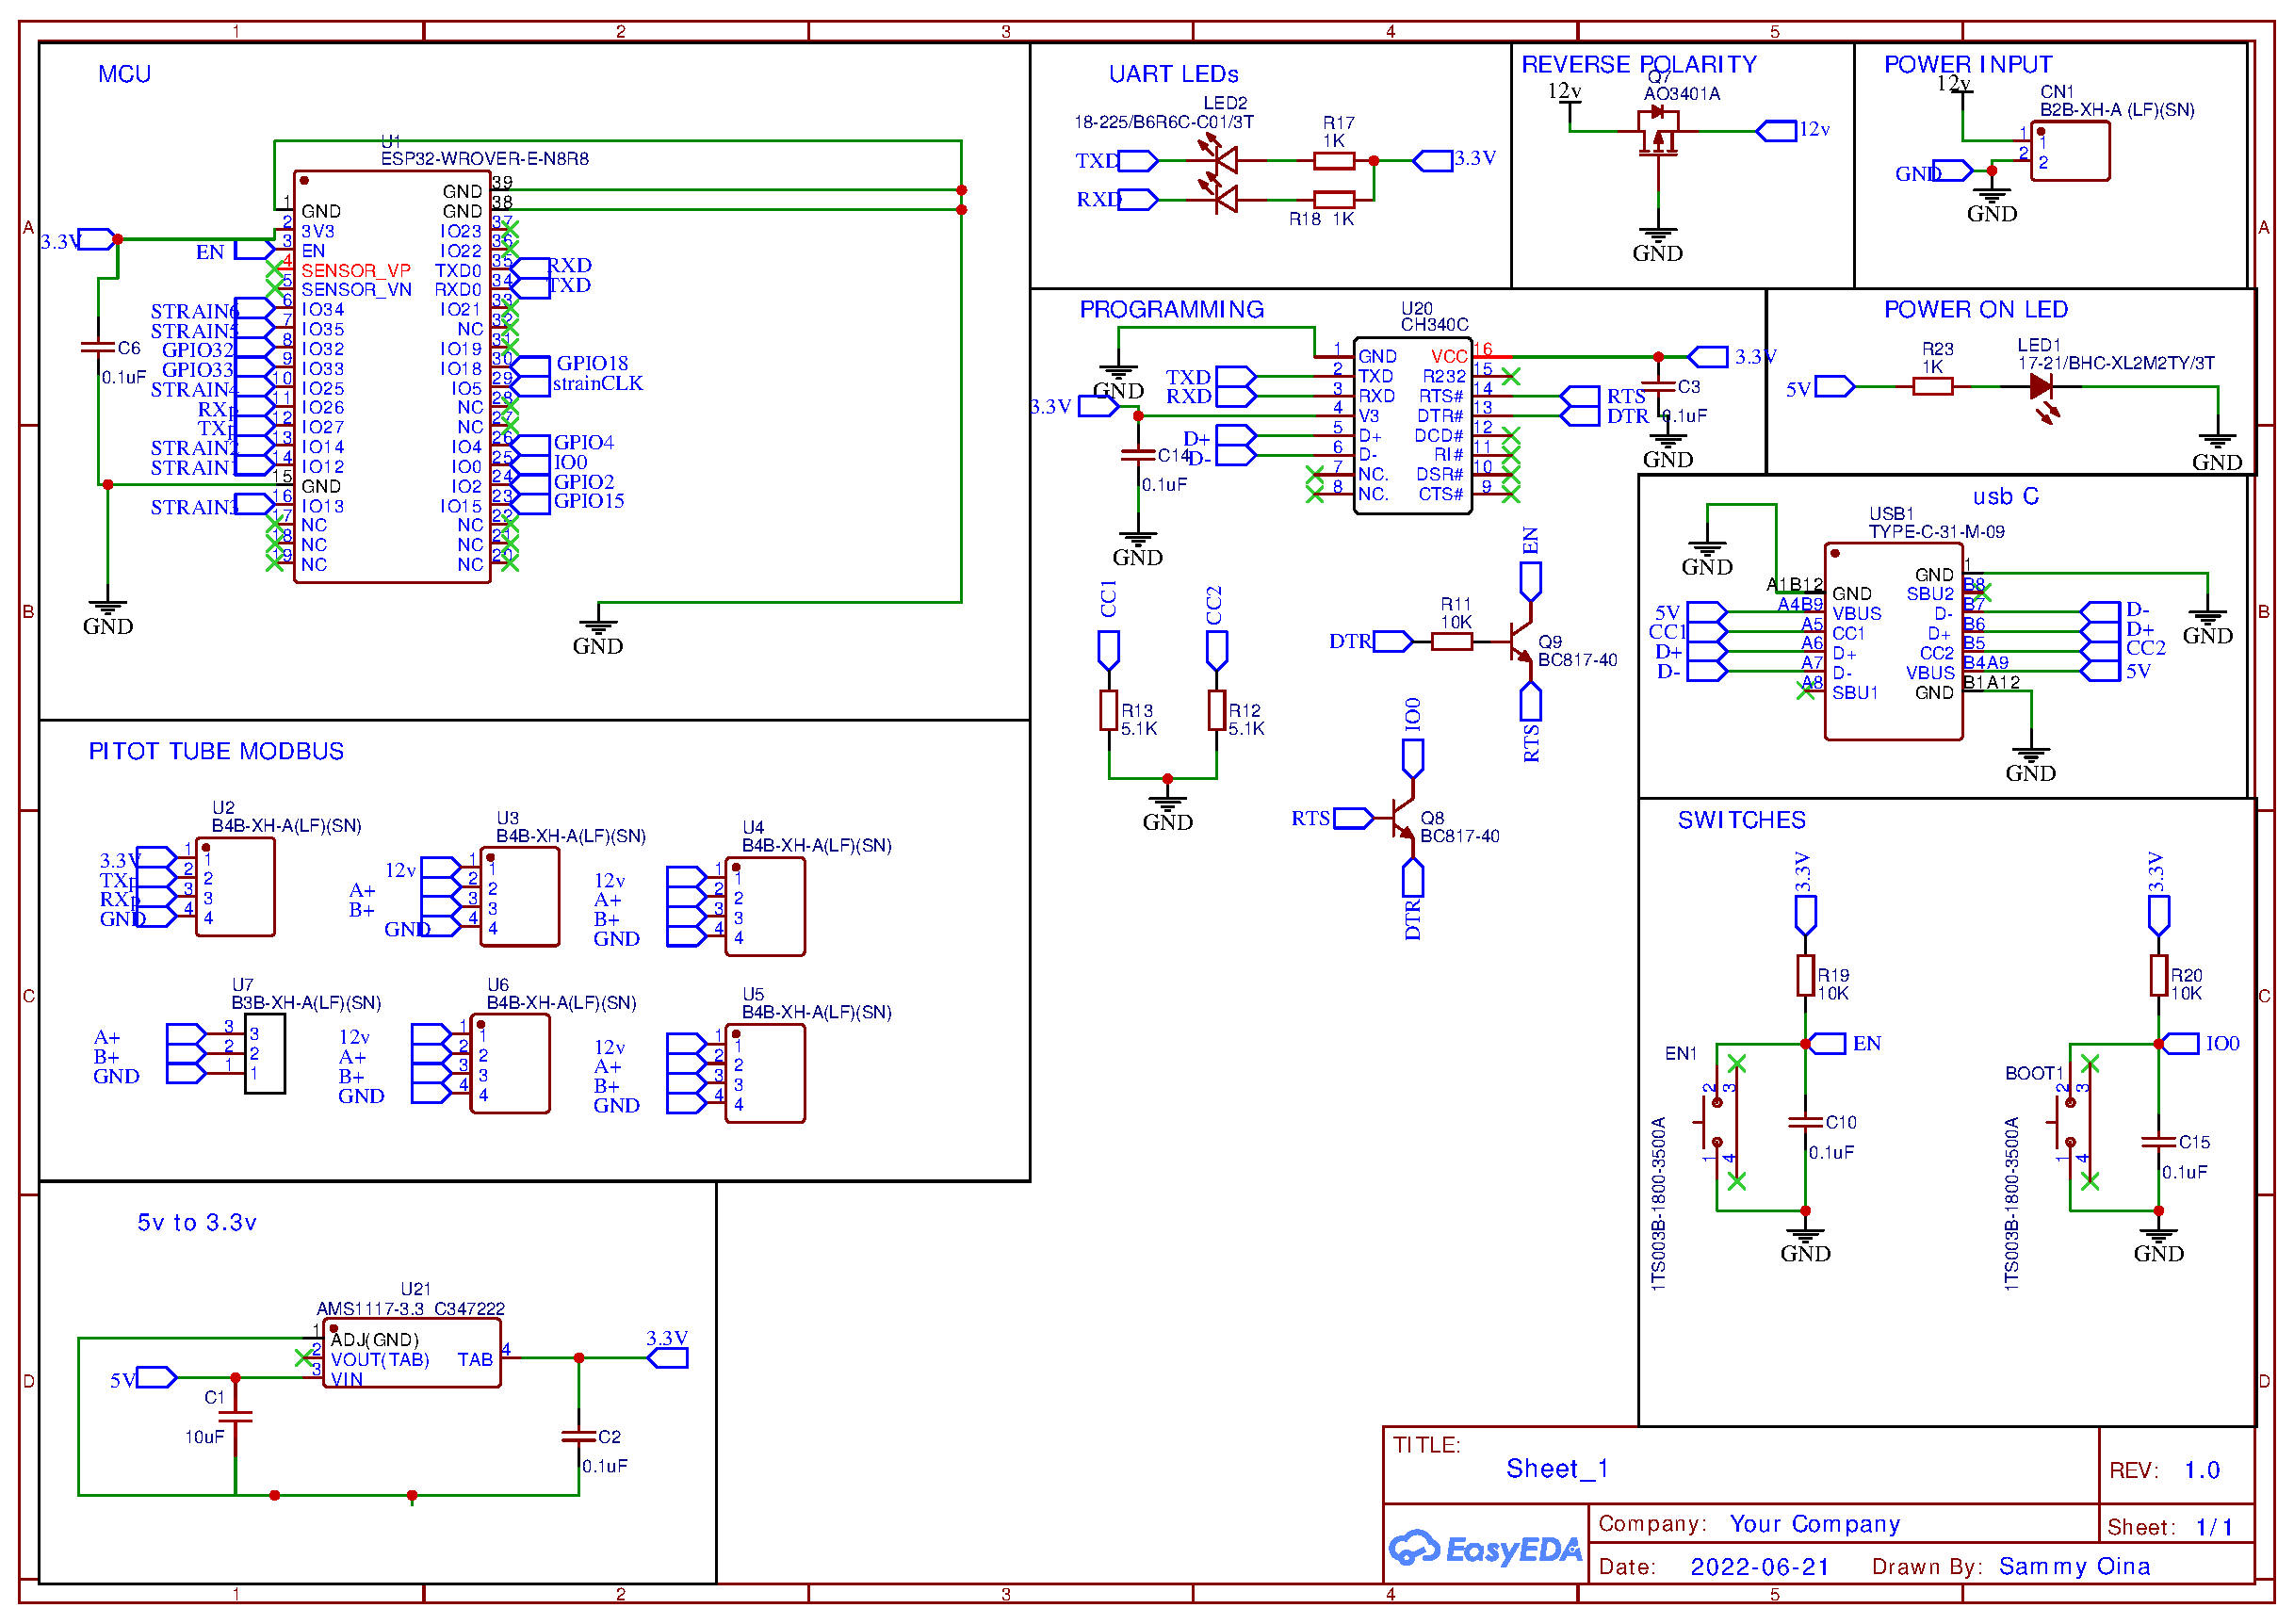
\includepdf[pages=-]{Figures/schm}
\end{document}